\documentclass[../main.tex]{subfiles}
\begin{document}
    \chapter{Research}\label{chap:research}

    The research is executed in 3 main steps.
    The first step creates an $M^3$ model for a PHP program and contains various facts about the program. 
    The creation of an $M^3$ for PHP is explained in more details in section \ref{sec:m3_for_php}.
    Once the $M^3$ model is constructed, the second step is to extract constraints from the program using the $M^3$ model. How and which constraints are extracted is described in section \ref{sec:fact_extraction}.
    In the third step, in section \ref{sec:research:constraint_solving}, the constraints are solved and resolve the types of variables used in the program.
    The final section \ref{sec:annotations} of this chapter explains how annotations can be included in the process to gain more precise results.
    
    \section{$M^3$ for PHP}\label{sec:m3_for_php}
    As explained in section \ref{sec:background_m3}, $M^3$ is a language independent meta model which holds facts about programs.
    The model can be extended with language specific elements and will be used to query the system for facts about the system.
    An overview how an $M^3$ for PHP is build is shown in figure \ref{fig:research_m3_creation}.
    Independent $M^3$ models are build each PHP file in the program.
    All these individual $M^3$'s are in the end combined to collect all the facts about a program.
    This results in one $M^3$ for the whole program.
    $M^3$'s are first created for each file is because it is not defined what the dependencies of a individual file are.
    There is no main file, and all files can load each other.
    In this research we assume that all files in a program are loaded when needed using autoloaders or manual includes.
    
    \begin{figure}[H]
        \centerline{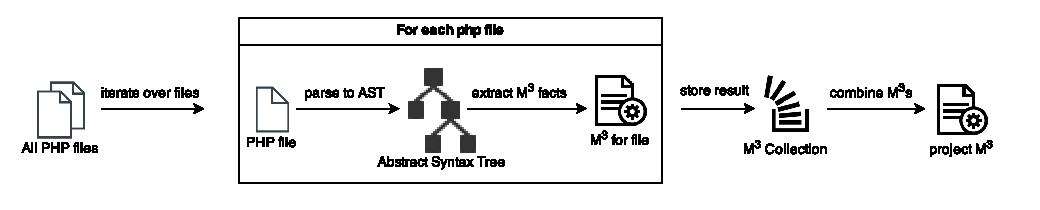
\includegraphics{Diagrams/M3Creation.pdf}}
        \caption{$M^3$ Creation}
        \label{fig:research_m3_creation}
    \end{figure}

    %The following steps are performed to create an $M^3$ for a system.
    %\begin{itemize}
    %    \item Parse all PHP files, resulting in an.
    %    \item For each file, create an independent $M^3$ from the ast.
    %    \item Combine all the m3s into one $M^3$ for the project.
    %    \item For each file, add additional informationNow run more analysis when all facts are collected in the m3. 
    %\end{itemize}
    
    \subsection{The algorithm}
    In order to get a better understanding of the creation of an $M^3$ for PHP, the algorithm is provided in Algorithm \ref{alg:research_m3}.
    \textbf{The input} of the algorithm is all the \texttt{PHP files of a program}, which are all files ending on \texttt{.php}.
    \textbf{The output} is an $M^3$ with facts about the provided program.
    The algorithm starts with initialising an empty $M^3$ collection in line \ref{alg:research_m3:init_collection} which with be filled with the result of each individual files.
    In the big loop on line \ref{alg:research_m3:loop_start} to \ref{alg:research_m3:loop_end} we iterate over all the PHP files of the program.
    The first thing that needs to be done is to create an Abstract Syntax Tree (\gls{AST}) of the program using an external PHP parser\footnotemark{} which returns an Rascal AST in \texttt{parseUsingPhpParserAndReturnRascalAST} on line \ref{alg:research_m3:get_ast}.
    \footnotetext{https://github.com/ruudvanderweijde/PHP-Parser}
    %In line \ref{alg:research_m3:add_modifier} we add ...
    From this AST we create an empty $M^3$ in \texttt{createEmptyM3} on line \ref{alg:research_m3:create_m3}.
    In order to be able to refer to any source code element, we need to have the declarations of the elements.
    These elements are extracted in \texttt{addDeclarations} on line \ref{alg:research_m3:add_decl} can be \texttt{namespace}, \texttt{class}, \texttt{interface}, \texttt{trait}, \texttt{method},  \texttt{function}, \texttt{variable}, \texttt{field}, or \texttt{constant}.
    For all \texttt{functions} we need to add scope information in case functions are declared inside another function or method.
    In line \ref{alg:research_m3:scope_info} we add the scope information to all nodes to the AST by visiting the AST.
    This is needed in order to extract the right facts about the logical containment which is done in line \ref{alg:research_m3:containment}.
    The next three lines (\ref{alg:research_m3:extends}-\ref{alg:research_m3:docblock}) extract facts about class inheritance and the interface implementations, modifiers, PHP doc blocks, and annotations.
    %In \texttt{calculateAliasesFlowInsensitive} on line \ref{alg:research_m3:aliases}
   	Once all the basic information is collected, \texttt{calculateUsesFlowInsensitive} on line \ref{alg:research_m3:uses} tries to find the declarations of the used objects, methods, functions and variables.
   	This is flow and context insensitive and only tries to resolve non-dynamic language constructs.
   	The last step of the iterator is to add the constructed $M^3$ to the $M^3$ collection.
   	Finally when an $M^3$ is constructed for all files, all facts of the individual $M^3$'s are merged into one $M^3$ model in line \ref{alg:research_m3:return}. 
   	\vspace{5 mm}
    \begin{algorithm}[H]
	 \KwIn{PHP files of a program}
	 \KwOut{$M^3$ for the PHP program}
     \BlankLine
	 m3Collection = []\;                                  \label{alg:research_m3:init_collection}
     \BlankLine
	 \ForAll{file $\in$ program}{                         \label{alg:research_m3:loop_start}
	  ast = parseUsingPhpParserAndReturnRascalAST(file)\; \label{alg:research_m3:get_ast}
   	  %ast = addPublicModifierWhenNotProvided(ast)\;      \label{alg:research_m3:add_modifier}
	  m3 = createEmptyM3(ast)\;                           \label{alg:research_m3:create_m3}
      \BlankLine
	  m3 = addDeclarations(m3, ast)\;                     \label{alg:research_m3:add_decl}
	  ast = addScopeInformation(m3, ast)\;                \label{alg:research_m3:scope_info}
      m3 = addContainment(m3, ast)\;                      \label{alg:research_m3:containment}
      \BlankLine
      m3 = addExtendsAndImplements(m3, ast)\;             \label{alg:research_m3:extends}
	  m3 = addModifiers(m3, ast)\;                        \label{alg:research_m3:modifiers}
	  m3 = addRawDocBlocksAndAnnotations(m3, ast)\;       \label{alg:research_m3:docblock}
      \BlankLine
	  %m3 = calculateAliasesFlowInsensitive(m3, ast)\;     \label{alg:research_m3:aliases}
	  m3 = calculateUsesFlowInsensitive(m3, ast)\;        \label{alg:research_m3:uses}
      \BlankLine
	  m3Collection += m3\;                                \label{alg:research_m3:add_to_collection}
	 }                                                    \label{alg:research_m3:loop_end}
	 \BlankLine
	 \Return projectM3 = composePhpM3(m3Collection)\;     \label{alg:research_m3:return}
	 \caption{PHP program to $M^3$}
	 \label{alg:research_m3}
	\end{algorithm}
    
    \subsection{Core elements}
    The $M^3$ model has the following core elements: \texttt{Declarations}, \texttt{Containment}, \texttt{Modifiers}, \texttt{Extends}, and \texttt{Uses}.
    All these core elements are explained in more detail in the paragraphs below.
    
    \paragraph{\texttt{Declarations}} defines the declarations of namespaces, classes, interfaces, traits, methods, functions, and variables and holds the relation between the logical name (which is used to refer to the declaration) and the actual file location (which is the physical place in the file system.
    For example the logical name of a class can be \texttt{$\vert$php+class://SomeNameSpace/ClassX$\vert$} while the actual location might be \texttt{$\vert$file:///project/SomeNameSpace/ClassX.php$\vert$}.
    
    \paragraph{\texttt{Containment}} holds information about what elements logically contain other elements.
    For example, a property or method is contained in a class and a class is contained in a package.
    When a function is declared in another function, they are both logically contained in the global namespace (the highers level) because all functions are declared as first class citizens in PHP.
    
    \paragraph{\texttt{Modifiers}} element contains information about the modifiers of classes, fields, and methods. 
    Classes can only be \texttt{abstract}, fields can be \texttt{public}, \texttt{private}, or \texttt{protected}, and methods can be all of them. 
    Abstract methods can only be declared in abstract classes. 
    Classes are implicitly public.
    
    \paragraph{\texttt{Extends}} contains information about what classes and interface extend other classes of interfaces. 
    Please note that we do not hold information about which class implements which interface, because that information is contained in the \texttt{implements} relation.
    Interface extensions work just like class extensions.
    
    \paragraph{\texttt{Uses}} relation holds information about the usages of certain elements.
    It is the relation between the usage and the declaration.
    For example when you instantiate a class, in that case you 'use' that specific class.
    
    \subsection{PHP specific elements}
    Because every programming language differs in syntax and semantics, the $M^3$ model is extensible to provide language specific modeling elements.
    The following php specific items are added: \texttt{Implements}, \texttt{TraitUses}, \texttt{Parameters}, \texttt{Constructors}, \texttt{Aliases}, and \texttt{Annotations}.
    These PHP specific modeling elements are described in more detail in the paragraphs below.
    
    \paragraph{\texttt{Implements}} holds information on what class implements which interfaces.
    One class can implement multiple interfaces.
    Because the information is a relation between the class and the interface, we can easily add multiple interfaces to one class in the model.
    
    \paragraph{\texttt{TraitUses}} knows which traits a class uses.
    Traits are a collection of reusable functions, are defined on class level, and one class can have multiple trait usages.
    All the methods of a trait are on runtime imported in the class.
    
    \paragraph{\texttt{Parameters}} keeps track of the parameters of a method or function.
    This information is stored to make it easier to resolve the call to a method or function.
    
    \paragraph{\texttt{Constructors}} lists all the constructors for classes. 
    This information is needed because it is not always clear what constructor is used, due to legacy PHP4 way of using class constructors.
    In PHP4 the constructor was defined as a method with the same name as the class.
    Since PHP5 the language is provided with a magic method \texttt{\_\_construct()}, which results in two ways to have constructors, but only one constructor will be called.
    The PHP4 constructors will be removed in PHP7.
    
    \paragraph{\texttt{Aliases}} has a relation between aliases and the actual implementation.
    For instance the function \texttt{class\_alias} defines a new name for the same class.
    This relation is also used to keep track of references. 
    
    \paragraph{\texttt{Annotations}} contain a relation between a declaration and the annotations that are known.
    Annotations are defined in the raw doc blocks and are parsed using regex.
    Regex was in this case easier then parsing because there is no official grammar or standard defined.
    For this research we only use \texttt{@param}, \texttt{@var}, \texttt{@returns}.
    
    \section{Fact extraction}\label{sec:fact_extraction}
    We extract fact about classes, class-constants, class-fields, methods, functions, and parameters.
    We store these facts in a relation in Rascal.
    The left side of the relation contains the class, function, or method.
    \\
    %todo: fact extraction (rewrite this stuff above, it totally makes no sense.
 
    Other facts that will be used:
    \begin{rascal} 
\CAT{Keyword}{alias} PhpParams = \CAT{Keyword}{lrel}{}[\CAT{Keyword}{loc} decl, \CAT{Keyword}{set}{}[\CAT{Keyword}{loc}] typeHints, \CAT{Keyword}{bool} isRequired, \CAT{Keyword}{bool} byRef];
\CAT{Keyword}{data} Annotation = returnType(\CAT{Keyword}{set}{}[TypeSymbol]) | parameterType(\CAT{Keyword}{loc} var, \CAT{Keyword}{set}{}[TypeSymbol])
    | varType(\CAT{Keyword}{loc} var, \CAT{Keyword}{set}{}[TypeSymbol]);

\CAT{Keyword}{anno} \CAT{Keyword}{rel}{}[\CAT{Keyword}{loc} from, \CAT{Keyword}{loc} to] M3@containment;          \CAT{Comment}{// 'from' directly contains 'to'}
\CAT{Keyword}{anno} \CAT{Keyword}{rel}{}[\CAT{Keyword}{loc} from, \CAT{Keyword}{loc} to] M3@extends;              \CAT{Comment}{// 'from' extends 'to' }
\CAT{Keyword}{anno} \CAT{Keyword}{rel}{}[\CAT{Keyword}{loc} from, \CAT{Keyword}{loc} to] M3@implements;           \CAT{Comment}{// 'from' implements 'to' }
\CAT{Keyword}{anno} \CAT{Keyword}{rel}{}[\CAT{Keyword}{loc} decl, PhpParams params] M3@parameters; \CAT{Comment}{// formal parameters of functions/methods}
\CAT{Keyword}{anno} \CAT{Keyword}{rel}{}[\CAT{Keyword}{loc} decl, \CAT{Keyword}{loc} to] M3@constructors;         \CAT{Comment}{// 'decl' and its constructor 'to'}
\CAT{Keyword}{anno} \CAT{Keyword}{rel}{}[\CAT{Keyword}{loc} decl, Annotation annotation] M3@annotations;  \CAT{Comment}{// result of parsed php docs}

    \end{rascal}
    
    \subsection{Type extraction}
    In order to define the subtype relations in class extensions, we will need to declare all existing class types.
    We can do this in rascal like is done in the example below:
    \begin{rascal}
\CAT{Keyword}{visit} (system) \{{}
    \CAT{Keyword}{case} c:class(\_{}, \_{}, \_{}, \_{}, \_{}): types += class(c@decl);
\}{}
    \end{rascal}
    Once all types are defined, we can add the subtype relation. We will need to have the subtype of \texttt{int()} and \texttt{float()} and the class extensions.
    You can see that in the code below:
    \begin{rascal}
\CAT{Keyword}{public} \CAT{Keyword}{rel}{}[TypeSymbol, TypeSymbol] getSubTypes(M3 m3, System system) 
\{{}
    \CAT{Keyword}{rel}{}[TypeSymbol, TypeSymbol] subtypes
        \CAT{Comment}{// add int() as subtype of float()}
        = \{{} \textless{}\textbackslash{}int(), float()\textgreater{} \}{} 
        \CAT{Comment}{// use the extends relation from M3}
        + \{{} \textless{}class(c), class(e)\textgreater{} | \textless{}c,e\textgreater{} \textless{}- m3@extends \}{}
        \CAT{Comment}{// add subtype of object for all classes which do not extends a class}
        + \{{} \textless{}class(c@decl), object()\textgreater{} | l \textless{}- system, /c:class(n,\_{},noName(),\_{},\_{}) \textless{}- system{}[l] \}{};
        
    \CAT{Comment}{// compute reflexive transitive closure and return the result }
    \CAT{Keyword}{return} subtypes*;        
\}{}
    \end{rascal}
  
    \subsection{Constraint extraction}
    (based on these rules, we can add constraints to the source code)
       
    Introduction is needed here... for now I will just list the types that I have found.
    Maybe this needs to be moved to a different chapter.
    \\
    \textbf{This is a list of items which are not supported (yet)}:

    \begin{itemize}
        
        \item References (in PHP they are symbol table aliases)
        \begin{itemize}
            \item on expression assignments :: $\$a \; = \; \&\$b$
            \item on functions :: function $\&f()$ $\{ \dots \}$
            \item on parameters :: function $f(\&\$a)$ $\{ \dots \}$             
        \end{itemize}

        \item Variable structures:
        \begin{itemize}
            \item \sout{Variable variables} :: $\$\$a;$
            \item \sout{Variable class instantiation} :: $new \; \$a;$
            \item \sout{Variable method or function calls} :: $\$a();$
        \end{itemize}

        \item List assign :: $list(\$a, \$b) = array("one", "two");$ (we can assume that the rhs is of type array, when the program is correct)
        
        \item \sout{Method or function parameters (including type hints)}
        \item \sout{Class structures, method calls}
        \item \sout{Class Constants}
        
        \item \sout{The global statement} (should be resolved by the usage relation from M3)
        
        \item \sout{Casts of expressions}
        
        \item Parameters
        
        \item \sout{Predefined variables} (\$this, self, parent, static)

        \item \sout{Eval} (will not be supported)        
        \item \sout{Closures} (not used much in production code)
        \item \sout{Traits} (not used much in production code)
        \item \sout{Callable} (introduced in 5.4 as typehint, not used much in production code)
        
        \item Foreach(\$a as ... (=> ...)) => \$a is an array or an object;
        \item \sout{return; => return type is null} (is added to the situation when there are no return statements)
        \item add predefined globals (and their type: \$[GLOBALS, \_SERVER, \_GET, \_POST, \_REQUEST, \_COOKIE, \_ENV, \_SESSION, php\_errormsg] (all in global scope))
        \item add magic constants: \_\_[DIR, FILE, LINE, NAMESPACE, FUNCTION, CLASS, METHOD]\_\_
        \item \sout{predefined constants: TRUE(b), FALSE(b), NAN(f), INF(f), NULL(n), STDIN(r), STDOUT(r), STDERR(r)}
        \item define("name", value) mixed with constants (?out of scope?)
        \item \sout{keywords: self, parent, static in a class} (is included in method and property calls    )
        \item ADD CONSTANTS! RECORD THE TYPE OF THE DEFINED CONSTANTS AND TRY TO READ THEIR TYPE.    
    \end{itemize}

    \hrulefill
    
    \textbf{Legend} \\
    \begin{table}[H]
        \begin{tabular}{ c c l c c l }
            $=$     & = & Equal to (type) &
            $C$     & = & A class \\
            $<:$    & = & Is subTypeOf &
            $\rightarrow c$     & = & A class constant \\
            $E_k$   & = & An expression &
            $\rightarrow p$     & = & A class property \\
            $[E_k]$ & = & Type of some expression &
            $\rightarrow m$     & = & A class method \\
            $f$     & = & A function &
            $[m]$   & = & (Return) type of a method call \\
            $[f]$   & = & (Return) type of a function &
            $(A_n)$ & = & The n'th actual argument \\
            $::c$   & = & Static property fetch &
            $(P_n)$ & = & The n'th formal parameter \\
            $::m$   & = & Static method call &
            $th$    & = & Type hint \\
            $::p$   & = & Static property fetch &
            $v$     & = & Default value \\
            Mfs     & = & Modifiers &
            $\Gamma$ & = & Whole program 
            
            
        \end{tabular}
        \caption{Constraint legend}
        \label{table:constraintLegend}
    \end{table}
    
    A list of predefined items can be found here:
    \begin{itemize}
        \item \href{Constants https://github.com/ruudvanderweijde/php-analysis/blob/master/src/lang/php/types/core/Constants.rsc}{Constants}
        \item \href{Constants https://github.com/ruudvanderweijde/php-analysis/blob/master/src/lang/php/types/core/Variables.rsc}{Variables}
        \item todo: functions
        \item todo: classes
    \end{itemize}

    
    \subsubsection{Expressions}
    \fact{assignment1}{Normal assignment}{}
    \fact{ternary}{Ternary}{}
    \fact{assignment2}{Assignments with operators (1)}{always resulting in ints}
    \fact{assignment3}{Assignments with operators (2)}{string concat ($.=$)}
    \fact{assignment4}{Assignments with operators (3)}{resulting in int where rhs is no array}
    \fact{assignment5}{Assignments with operators (4)}{resulting in int or float}
    \fact{unaryOperators}{Unary operators}{}
    \fact{binaryOperators}{Binary operators}{}
    \fact{comparisonOperators}{Comparison operators}{}
    \fact{logicalOperators}{Logical operators}{}
    
    \subsubsection{Array}
    \fact{arrayAccess}{Array value fetch}{}
    \fact{array}{Array declaration}{}

    \subsubsection{Scalars}
    \fact{scalar}{Scalars}{}
    \fact{encapsed}{Encapsulated strings}{}
    
    \subsubsection{Casts}
    \fact{casts}{Casts}{\\ {\footnotesize{Note: PHP Warnings are ignored}}}
            
    \subsubsection{Clone}
    \fact{clone}{Clone}{}
    
    \subsubsection{Class}
    \fact{instantiation1}{Class instantiation (1)}{matching the class name}
    \fact{instantiation2}{Class instantiation (2)}{of an expression}
    \fact{keywords}{Special keywords}{\texttt{self}\, \texttt{parent} \texttt{parent} \texttt{static}}
    \fact{property1}{Class property fetch}
        {\\ \footnotesize{* Possible add fact that the field E is declared in class C, when it is on the left side of an assignment.}}
    \fact{property2}{Class property fetch variable}{}
    \fact{methodCall1}{Class method call}{}
    \fact{methodCall2}{Class method call variable}{}
    \fact{classConstants}{Class constants (needs to be reviewed)}{}
    
    \subsubsection{Parameters}
    \fact{parameter1}{Parameters in class instantiation}{
        \\
        \footnotesize{*These parameters are just examples for what happens if they have typeHints ($th$), default values($v$) or none}
        \footnotesize{*The constructor can be found in the m3 model (@constructors(loc classDecl, loc constructorMethodDecl))}
    }
    
    \subsubsection{Scope}
    \fact{function1}{Type of a certain variable within some scope}{\\ {\footnotesize{this applies to global- class- function- and method- scope}}}
    \fact{return1}{Return type of function or method (1)}{having no return statements or \texttt{return;}}
    \fact{return2}{Return type of function or method (2)}{every exit path ends with a return statement}
    \fact{return3}{Return type of function or method (3)}{possible no return value}
    
    \subsubsection{Function calls}
    \fact{functionCall1}{Function call}{}
    \fact{functionCall2}{Function call variable}{}
    
    How to resolve expressions:
    \begin{itemize}
        \item Find all expressions which are defined above and annotate them with @type.
        \item Annotate the rest of the expressions with @type = any(); (should only be for relevant expressions)
    \end{itemize}
    
    \section{Constraint solving}\label{sec:research:constraint_solving}
    When we have all the constraints from the source code as facts, we will solve the constraints until we can no longer solve any constraints.
    The result will be a list of possible types for each class, method, fields, functions, variable and expression.
    \\
    The first step is to initialise all type-able objects we want to solve.
    In this initial phase the status of all objects can be of any type, because we do not know anything about them yet.
    When we solve the constraints step by step, we will be able to limit the number of possible types for a certain object.
    We do this by taking the intersection of the constraint result and the possible types we have.
    This way there should be less and less possible types for each variable.
    \\
    When we take the intersection of none overlapping types, we have a type error.
    There is no possible type for this object.
    Because PHP allows ducktyping, allowing objects to be of more than one type, we will use widening in these cases.
    Widening means that we pick the union instead of the intersection, so we can continue our analysis.
    \\
    Some of the constraints only give us information that a certain object should be a subtype of a certain type.
    When we solve these constraints, we will take the least common ancestor.
    
    \section{Annotations}\label{sec:annotations}
    %todo: moved this section below constraint solving: check copy
    After we gathers all the facts from the source code, we will add additional information which we read from the annotations.
    For this we use regex to match \texttt{@return type} and \texttt{@param type var} for methods and functions.
    We read \texttt{@var type} for variables and class attributes.
    In our first analysis we do not include the facts we gathered from the annotations. 
    In the second analysis we do include the facts.
    This way we can compare the end results.
    \\
    In order to gain some knowledge about the reliability of the annotations, we compare the result our or initial analysis with the provided provided annotation information.
    Here the implementation should comply to the used annotations.
        
\end{document}
